\chapter{Implementation}\label{cha:implementation}
This chapter covers the implementation of the Arc programming language. This includes a model of the compilation process and the compilation target, a short discussion of the visitor pattern, and a look at the implementation of the visitors, symboltable, typechecking, and scopechecking.


\section{Compiler}\label{sec:compiler}
The purpose of a compiler is to convert source code into target code. A generalized model of the compilation process can be seen in Figure~\ref{fig:generalcompilermodel}. In the case of the Arc compiler, the source code is text written in the Arc language.


\begin{figure}[htb!]
    \centering
    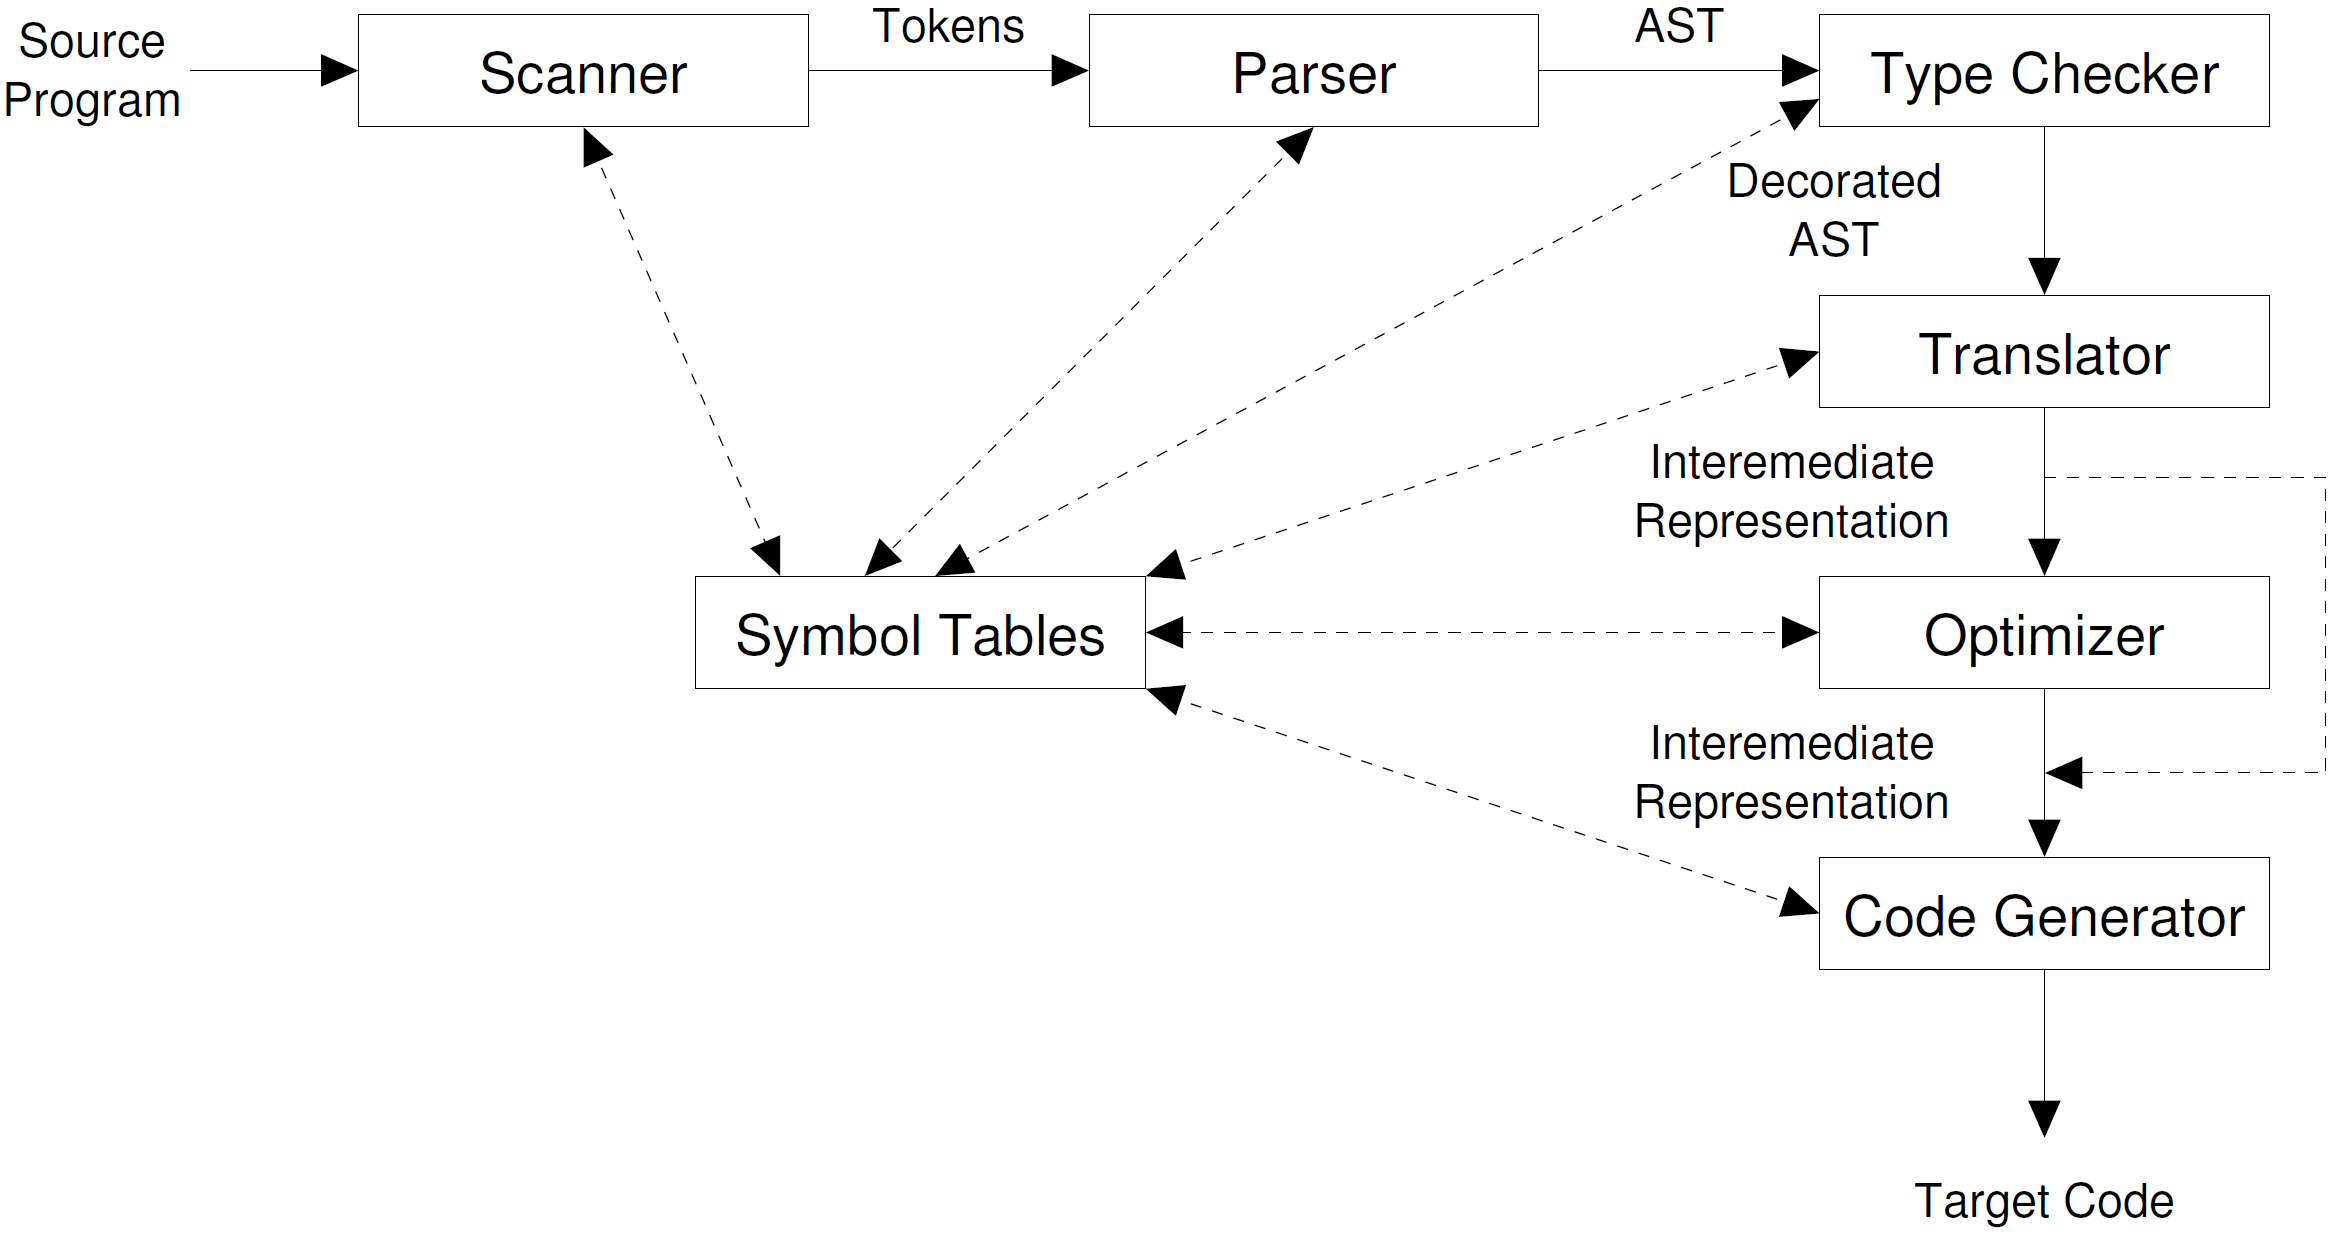
\includegraphics[width=0.8\textwidth]{figures/Full_Compiler.png}
    \caption{A textbook example of a compiler~\cite{CraftingCompiler}}
    \label{fig:generalcompilermodel}
\end{figure}


The target code is often low-level code for a particular system or runtime, but not always. When the target code is another high-level language, the process is also called transpilation. The Arc language is used for programming Arduinos, and so the compiler has to either generate Arduino-specific machine code or transpile it to the high-level Arduino language. Because the Arc language leverages the Protothreads library and its concurrency model for the Arduino, it makes sense for the Arc compiler to be a transpiler.

The Arc compiler follows many of the steps of the general model. Figure~\ref{fig:arccompilermodel} models the Arc compiler with some essential details.


\begin{figure}[htb!]
    \centering
    \begin{tikzpicture}[node distance=3cm]
        \begin{scope}[node distance=3cm,local bounding box=clusterA]
            \node (a) [state] {Scanner} node[below,scale=.7, xshift=60,yshift=-20]{Antlr};
            \node (b) [state, right of=a] {Parser};
            \draw[arrow, ->] (a) -- node[above,scale=.70,align=center]{Tokens} (b);
        \end{scope}
        \begin{scope}[node distance=3cm,local bounding box=clusterB]
            \node (c) [state, shift={($(b.east)+(2.3cm,0)$)}] {Type checker} ;
            \node (d) [state, shift={($(c.south)+(0,-1.5cm)$)}] {Scope checker};
        \end{scope}
        \node(clusterA_g)[cluster,fit=(clusterA)]{};
        \node(clusterB_g)[cluster,fit=(clusterB)]{};
        \node (q) [state, below of=clusterA_g] {Symbol table};
        \node (e) [state, shift={($(d.south)+(0,-1.5cm)$)}] {Code generator};
        \node (f) [shift={($(e.south)+(0,-1cm)$)}] {Target code};
        \node (start) [shift={($(clusterA.west)+(-2cm,0)$)}] {Source code};
        \draw[arrow, ->] (start) -- (clusterA_g);
        \draw[arrow, ->] (b) -- node[right,scale=.70,xshift=-16,yshift=7]{AST} (c) node[below,scale=.7, xshift=-30,yshift=-25, align=left]{Contextual\\ analysis};
        \draw[arrow, ->] (c) -- node[right,scale=.70,align=center]{AST} (d);
        \draw[arrow, ->] (d) -- node[right,scale=.70,align=center]{AST} (e);
        \draw[arrow, ->] (e) --  (f);
        \draw[arrow, dotted, <->] (q) --  (clusterB_g);

    \end{tikzpicture}
    \caption{The Arc compiler model.}
    \label{fig:arccompilermodel}
\end{figure}


Figure~\ref{fig:arccompilermodel} shows how the source code is first scanned into tokens and then parsed into an \gls{ast}. \gls{antlr} generates the lexer and parser for this from our grammar, hence the box around the scanner and parser. The \gls{ast} is then type-checked and scope-checked. The type and scope check rules are explained in more detail in section~\ref{sec:contextualconstraints}. Once the transpiler has done all of the necessary checks on the source code, it is ready to generate the Arduino code, which is also the final step of the compiler. The target code is now ready for the Arduino bases on the source code.
\section{Lexer and parser generation}

%what the lexer and parser is
%differences
%how it is used
%why it is used
%how we generate them
%alternatives
This section will briefly cover how the lexer and parser for Arc has been implemented, and what alternatives could have been used.

For Arc, \gls{antlr} has been used, for creating the grammer and also to generate both the lexer and parser. From writing the grammar, is was possible for \gls{antlr} to generate the lexer, parser and more.\cite{Parr2014} This made \gls{antlr} highly effective for designing Arc, as small changes to the grammar could easily be made, without having to re-create the lexer and parser everytime. Instead only the grammar had to be changed, and \gls{antlr} would generate a new lexer and parser, based on the new grammar.

The grammar was made in a file called 'arcv2.g4' which is an \gls{antlr} file, that \gls{antlr} recognizes and also the lexical rule were made in a file called 'lexerRules.g4'. With these files, \gls{antlr} could generate all needed files for the parser, the lexical analyzer, and other supporting files. These files can be seen in the image \ref{fig:lexerandparserfiles}

\begin{figure}[htb!]
    \begin{center}
        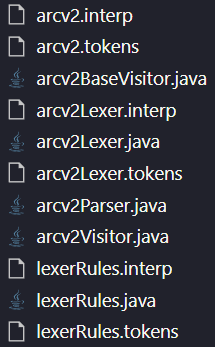
\includegraphics{figures/lexerAndParserFiles.png}
        \caption{Files generated for Arcs parser and lexical analyzer}
        \label{fig:lexerandparserfiles}
    \end{center}
\end{figure}

Figure \ref{fig:lexerandparserfiles} shows all files that \gls{antlr} generates, from the grammar rules and lexical rules. The file 'arcv2Parser.java' is the parser.\todo[]{Describe how the parser works and how it is used. Show code example!}


Another option to this could have been by writing out both the parser and lexer by hand, this could be very educational, as creating our own parser and lexer, would give in-depth knowledge of how they each work. But this would increase the time needed to create Arc considerably as, as mentioned previously, any minor change made in the grammar, would also mean going through the lexer and parser to fix them accordingly. This could lead to time wasted, which is a limiting factor for this project. Therefore it was decided to use the obviouse solution, to use the tools that readily avaliable. For this reason in particular, using \gls{antlr} to generate the lexer and parser for us, was the obviouse choice. 



\todo[inline]{Consinder adding examples of how we specifically have done it and discuss the files generated}

%The lexer, also called a lexical analyzer or scanner, takes a character stream and turns it into tokens. Tokens are a representation of something in a language, such as a num in Arc would be a token, that represents numbers. The lexer recognizes and can discard tokens of the character stream, so that the parser can ignore them. This includes tokens such as comments and whitespaces, that the parser does not need to concern itself with. If the lexer did not discard these tokens, that parser would constantly have to check for them. These tokens are then passed to the parser, that makes syntatic sense of them. It compares the tokens and their structure to the grammar of the specific language.\cite{Parr2014}



\section{Visitor pattern}\label{sec:visitorpattern}\feedback{We still working on this section, and unsure what }
This section will briefly discuss what the visitor pattern is, how it is used in Arc, and why it is used. ANTLR provides two methods of traversing a \gls{cst}, listeners and visitors. 

The listener pattern, is not responsible for calling methods to traverse the tree. ANTLR generates enter and exit methods for each rule, these methods are then called when the walker encounters a node. The benefits of using the listener pattern, is that it is automatic, and the methods created do not have to explicitly visit all their child nodes\cite{Parr2014}. \feedback{We are unsure of how correct this actually is, taken from: Page 18}

The visitor pattern, is a method used to traverse the \gls{cst} in a specific manner, where methods are used to visit each child node. By using the visitor pattern, there is more control of how the traversal of the \gls{cst} is done, and how much of the \gls{cst} is visited. ANTLR can generate a visitor interface, this interface is created from Arcs grammar, and creates all the needed visitor methods. These act as boilerplate for Arcs needed visitor methods, that can then be written out to do excatly as needed\cite{Parr2014}. 

For Arc there is made use of the visitor pattern, because it is not neccecary, for Arc, to visit all nodes, since for some of them it is know what will follow. It is also the more secure option, as it gives the option to be more specific about what happens for each node. This is especially good for futureproofing, as there might be certain things that had not been prdicted, and can therefore be specifically fixed.


%Options
%pros and cons of both
%How is it used
%How do we use it


%Vi vil ikke altid ind i alle noder, fordi det ikke er nødvændigt
%Det er sikre valg, da vi kan være specifikke for hver node, hvis der er noget vi ikke har forudset
%Future proof





\section{MOVE ME EVENTUALLY}
This section contains text that has to be moved to proper sections.

\subsection*{Arc implemementation of the sample project}
The sample project implemented in Arc.

\begin{listing}[htb!]
    \begin{minted}[label=Arc example]{text}
        #pin BUTTON_PIN(12, OUTPUT);
        mut num buttonState = 0;
        mut bool ledState = HIGH;

        task(bool ledState) every 1000 {
            ledState = !ledState;
            digitalWrite(LED_BUILTIN, ledState)
        }

        task(num buttonState) {
            buttonState = digitalRead(BUTTON_PIN);
            Serial.Println(buttonState);
        }
    \end{minted}
    \caption{Project example implemented in Arc, assuming print is possible.}
    \label{lst:arcexample}
\end{listing}
